
\section{Background}

\subsection{FaaS Function Execution} % Cold-starts and Keep-alive}

\noindent \textbf{Function Initialization Overheads.}
The Function-as-a-Service computing paradigm sees providers running user code on-demand when a request comes in, and importantly deciding \emph{where} it should run. 
Each invocation must be run in isolation from other concurrent and co-located invocations, and thus security isolation is provided by running each invocation in a fresh sandboxed environment. 
Sandboxes are generally implemented using containers (such as Docker~\cite{docker-main}) or lightweight VMs (such as Firecracker~\cite{firecracker-nsdi20}) created on the server that runs the invocation.
Creation time for both choices can be significant, adding latency to the in-flight request. 

Many techniques have been proposed to reduce the initialization overhead from such \emph{cold starts}.
Cold starts  can be mitigated by skipping initialization entirely, by saving in memory and reusing the execution environment for subsequent invocations of the same function. 
Keeping the function ``warm'' thus allows a provider to amortize the startup cost across future invocations. 

The warm and cold time for different functions from the FunctionBench \cite{kim_functionbench_2019} workload suite are shown in Table~\ref{tab:func-times}.
The table shows the total execution latency when these functions are run on OpenWhisk.
The cold times, because of the large initialization overheads, are $1-10\times$ larger than the warm running time, which occurs when the function is run in an already initialized container which is cached in memory. 

\begin{table}
  \begin{tabular}{ c c c }
\hline
  Application & Warm Time (s) & Cold Time (s) \\ 
\hline
  Web-serving & 0.179 & 1.153 \\  
  ML Inference (CNN) & 2.211 & 7.833 \\
  Disk-bench (dd) & 1.068 & 2.944 \\  
  % float & 0.083 & 1.432 \\  
  % gzip & 0.406 & 1.033 \\  
  % image & 4.806 & 5.268 \\  
  Matrix Multiply & 0.117 & 1.067 \\  
  Sklearn Regression & 53.57 & 54.45 \\  
  AES Encryption & 0.587 & 2.064 \\  
  Video Encoding & 10.28 & 11.51 \\  
  JSON Parsing & 0.414 & 1.962 \\
\hline
\end{tabular}
\caption{FunctionBench \cite{kim_functionbench_2019} functions run times' are significantly longer on cold starts. Ideally we want all of our functions to run warm to lower user latency. Cold starts also increase system load by creating runtime overhead.}
\label{tab:func-times}
\vspace*{-0.4cm}
\end{table}


% Table should be here? 
% Multiple containers for a function can exist, but they ultimately must reside on some specifc server(s).
% To encourage reuse for lower latency, the provider must have a load balancing policy that ensures \emph{locality}. 
% Consistently routing a function to the same server reinforces the warm container and improves response time and system latency. 

\noindent \textbf{Keep-Alive for reducing cold-starts.}
% An individual server impacts latency by choosing when and which functions to keep warm in memory.
Servers cannot keep all the functions routed to them in memory indefintely, and when memory is needed it must choose which to retain, aka a \emph{keep-alive} policy.
Many FaaS offerings, including OpenWhisk which we build on here, use a time-to-live approach that \emph{evicts} a function from memory if it isn't used within a certain time window.
%
% When the server removes the function container from memory it has been \emph{evicted}.
More recent advanced techniques based on LRU and GreedyDual~\cite{gdsf} caching algorithms make the decision based on the functions startup time, memory footprint, and invocation frequency when making evictions~\cite{faascache-asplos21}.

However, the benefits of locality have been investigated primarily at the \emph{single-server} level.
Most real-world FaaS deployments use a large cluster of servers sitting behind a load-balancer.
Tailoring the load balancing algorithm to compliment the choices made by the cache eviction algorithm, especially locality reuse, is vital in FaaS, and is the focus of this paper.
For example, ``sticky'' load-balancing and routing a function to the same server preserves locality, but at the risk of a highly overloaded server.
Since function latencies also depend on the load on the server, this naive policy would be sub-optimal, especially if the workload consists of functions with highly variable popularities and running times.
We shall elaborate on this further in the next section, and show that the tradeoffs imposed by FaaS requires a new class of load-balancing approaches. 


% Regardless, if a server makes good eviction choices it results in warm runs by keeping functions more likely to be invoked (i.e. \emph{cache hits}) and poor eviction choices lead to \emph{cache misses}.

% Each invocation: new container or lightweight VM created.
% This can take significant time, contributing to function latency. 
% The additional overhead of non-function parts need to be avoided.
% % Can we add new figure? or table?

% \paragraph{Function Initialization Overheads.}
% For instance, the virtual execution environment can take 100s of ms to start up.

% Violin-plot figure here... 

% \paragraph{Keep-Alive for reducing cold-starts.}
% Many techniques have been proposed to reduce the initialization overhead.
% One common general technique is to keep the initialized container state in server memory, and serve the subsequent invocations of the same function from this pre-initialized container.
% Thus keeping functions alive can amortize the function initialization overheads. 


% Thus \emph{locality} is a key principle.

% Cache hits and misses. 
\vspace*{-0.2cm}
\subsection{Load Balancing}

Managing the load of a cluster of servers is a common problem in distributed computing systems.
Load-balancing policies typically rely on some notion of ``load'' of a server, such as the number of concurrently executing tasks, length of the task-queue, cpu-utilization, etc.
%
The first broad class is \emph{compute-oriented} load-balancers, typically used for short-running tasks and queries. 
Load-balancing for computational tasks is common in scenarios like web-clusters~\cite{karger1999web}. 
In these systems, the tasks can be executed on any server,  servers in a cluster are largely fungible, and the task performance largely depends on the server-specific cpu-utilization at the time.

Load-balancing techniques have received significant theoretical attention (especially using queuing theory), as well as many practical systems~\cite{decandia2007dynamo}. 
From a queuing theory perspective, policies such as least-work-left (LWL) and Join-Shortest-Queue (JSQ), have studied near-optimal load balancing for computing load-dependent workloads under a processor-sharing (PS) setting. 

Interestingly, load-balancing for \emph{data-oriented} systems, such as Content Delivery Networks (CDNs)~\cite{nygren2010akamai}, and distributed key-value stores (such as Amazon Dynamo~\cite{decandia2007dynamo}) must also balance the load on servers, but with data locality as a key requirement.
In this context, locality refers to requests for the same object being handled by the server, or the same subset of servers if the object is replicated. 
We find that FaaS load balancing requires and benefits from \emph{both} these objectives: minimizing computing load \emph{and} maximizing locality to reduce cold-starts. 

\begin{comment}
However, combining compute-oriented load-balancing solutions 

In large clusters, consistent load information cannot always be assumed, and simple techniques work well in practice.
For instance, the power of two random choices, which schedules a task on the least loaded of two random servers. 

Queuing analysis?
- G/G/PS system. Greedy load balancing is sub-optimal.

Randomization and power of 2 choices is popular.

But arent locality aware.

Web server load balancing work. A Gandhi etc. 
\end{comment}

\vspace*{-0.2cm}
\subsection{Consistent Hashing} 
\label{subsec:ch}

\begin{figure}
  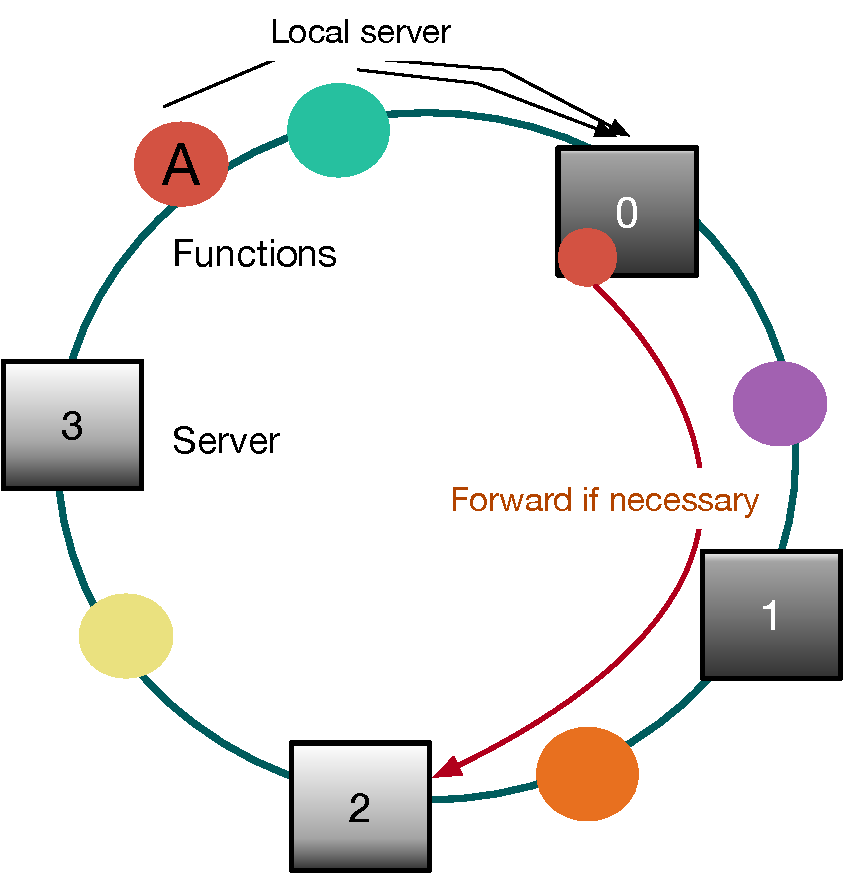
\includegraphics[width=0.3\textwidth]{../figs/ch-bl.pdf}
  \vspace*{-0.2cm}
  \caption{Consistent hashing runs functions on the nearest clockwise server. We forwards them if  server is overloaded.}
  \label{fig:ch}
    \vspace*{-0.2cm}
\end{figure}

For data-oriented systems, a common technique to ensure locality is Consistent Hashing~\cite{karger1999web, karger1997consistent}.
Objects are mapped to servers based on some object id or key.
Consistent hashing preserves object-server mapping even in the face of server additions and removals, which improves locality.
%
Figure~\ref{fig:ch} provides an overview of consistent hashing. Both objects and servers are hashed to points on a ``ring'', and objects are assigned to the next server (in the clockwise direction) in the ring. 
Addition or removal of servers only affects the nearby objects by remapping them to the new next server in the ring.

OpenWhisk uses a modified consistent hashing algorithm for its default load balancer.
As functions are sent to servers, their expected memory footprint is added to a server-specific running counter of outstanding requests.
Upon completion the memory size of a function is decremented from that server's counter.
If the counter for a function's ``home'' server would exceed the assigned memory on the server it is forwarded along the ring.
%
The drawback of this policy, and consistent hashing as a whole, is that the performance can be affected by the relative popularities of the different objects.
A highly popular object can result in its associated server getting overloaded.
This problem is exacerbated in the case of FaaS functions, as we shall demonstrate in the next section. 


%%% Local Variables:
%%% mode: latex
%%% TeX-master: "paper"
%%% End:
